\documentclass[12pt,a4paper]{ctexart}

\usepackage{geometry}
\usepackage{graphicx}
\usepackage{array}
\usepackage{booktabs}
\usepackage{amsmath}
\usepackage{xeCJK}
\usepackage{tikz}
\usepackage{titlesec}

% 页面设置
\geometry{
    top=2.5cm,
    bottom=2.5cm,
    left=2.8cm,
    right=2.8cm
}

% 定义 section* 格式
\titleformat{\section}
  {\zihao{-3}\heiti\bfseries}
  {}
  {0em}
  {}
\titlespacing*{\section}{0pt}{0.5cm}{0.3cm}  % 左缩进、上间距、下间距


% 取消页码（封面）
\pagestyle{empty}

% 定义等长下划线命令（固定宽度 6.5cm，左对齐）
\newcommand{\infofill}[1]{{\zihao{4}\songti\underline{\makebox[6.5cm][c]{#1}}}}

% 定义内容区块命令
\newcommand{\reportsection}[2]{%
    \noindent{\zihao{-3}\heiti\bfseries #1（#2分）}
    \vspace{0.3cm}
    
    \noindent\rule{\textwidth}{0.4pt}
    \vspace{6cm}
}

% 设置中文字体
\setCJKmainfont{SimSun}  % 宋体，可根据系统改为 Noto Serif CJK SC 等

\begin{document}
% ==================== 封面页 ====================
\begin{titlepage}
    \centering
    \vspace*{1.5cm}
    % 校徽占位（正方形示例图）
    
\includegraphics[width=5cm,height=5cm]{images/image-2026-09-07-14-57-04.png}
    
    \vspace{1.8cm}
    
    % 中山大学
    {\zihao{1}\heiti\bfseries 中山大学}
    
    \vspace{0.9cm}
    
    % 微电子科学与技术学院
    {\zihao{2}\heiti 微电子科学与技术学院}
    
    \vspace{0.9cm}
    
    % 课程名称
    {\zihao{2}\heiti 《集成电路元器件特性表征实验》}
    
    \vspace{0.9cm}
    
    % 实验报告
    {\zihao{1}\heiti\bfseries 实验报告}
    
    \vspace{3cm}
    
    % 信息表格
    

    % 信息表格（无任何框线，无横线，无竖线）
    \begin{tabular}{@{}>{\zihao{4}\heiti}r @{\hspace{1.2em}} l@{}}
        实验主题      & \infofill{半导体禁带宽度测试}        \\[0.8cm]
        姓\quad\quad 名 & \infofill{徐睿琳}   \\[0.8cm]
        学\quad\quad 号 & \infofill{23342107} \\[0.8cm]
        实验日期      & \infofill{\today}   \\[0.8cm]
    \end{tabular}
    
    \vfill
\end{titlepage}

% ==================== 内容页 ====================
\newpage
\pagestyle{plain}
\setcounter{page}{2}

% 导言区需加载：\usepackage{ctex,amsmath,geometry}

\section*{实验目的（5分）}
\begin{enumerate}
  \item 了解紫外--可见--近红外分光光度计的内部构造与各元件功能（光源、单色器、斩光镜、探测器等）；
  \item 掌握光吸收系数法测定半导体光学禁带宽度的原理及 Tauc 外推法的数据处理流程；
  \item 测定钙钛矿薄膜与硅晶圆的吸收光谱，判别其跃迁类型（直接/间接带隙）并求取禁带宽度 $E_g$。
\end{enumerate}

\section*{实验原理（10分）}

晶体中电子处于能带态，价带顶 $E_v$ 与导带底 $E_c$ 之间不存在公有化运动状态，该能量间隔即禁带宽度
$E_g=E_c-E_v$，它决定了本征载流子浓度与材料的导电特性。当入射光子能量满足 $h\nu \ge E_g$ 时，价带电子
吸收光子发生带间跃迁，吸收系数 $\alpha$ 在吸收边附近急剧上升，据此可由吸收边位置确定 $E_g$。

假设价带与导带近似为抛物线、跃迁矩阵元与光子能量无关，带间跃迁吸收系数满足 Tauc 关系
\begin{equation}
  (\alpha h\nu)^{1/n}=B\,(h\nu-E_g),
  \label{eq:tauc}
\end{equation}
其中 $B$ 为比例常数，$n$ 由跃迁类型决定：直接带隙半导体（如 ZnO、钙钛矿）取 $n=1/2$，电子跃迁无需声子
参与动量补偿；间接带隙半导体（如 Si）取 $n=2$，跃迁需声子参与以满足动量守恒，故吸收边较为平缓。

分光光度计直接测得的是吸光度 $A$ 与波长 $\lambda$ 的关系。由朗伯--比尔定律 $A=K\alpha$（$K$ 为与
$\alpha$ 无关的常数），代入式 \eqref{eq:tauc} 得
\begin{equation}
  (A h\nu)^{1/n}=C\,(h\nu-E_g),\qquad C=BK^{1/n}.
  \label{eq:tauc_A}
\end{equation}
以 $(A h\nu)^{1/n}$ 为纵坐标、$h\nu$ 为横坐标作图，式 \eqref{eq:tauc_A} 即直线 $y=C(x-E_g)$，其在横轴
上的截距即为 $E_g$。光子能量由波长换算
\begin{equation}
  h\nu=\frac{hc}{\lambda}\approx \frac{1240}{\lambda}\;(\mathrm{eV}),\quad \lambda\ \text{以 nm 计}.
\end{equation}

数据处理时，直接带隙作 $(A h\nu)^2$--$h\nu$ 图、间接带隙作 $(A h\nu)^{1/2}$--$h\nu$ 图，选取吸收边附近
线性段作最小二乘拟合，令 $y=0$ 求得的 $x$ 截距即为禁带宽度。测试前进行基线校正，用以扣除衬底吸收、界面
反射与散射以及仪器光谱响应的影响。

\section*{实验设备和步骤（5分）}

\textbf{实验设备：}岛津 SHIMADZU UV-3600i Plus 紫外--可见--近红外分光光度计，配 50\,W 卤素灯与氘灯双光源、
双单色器（光栅 G1--G4）、斩光镜（样品/参比双光束）及 PMT（紫外--可见）、InGaAs（近红外--短波红外）、
PbS（短波红外）三探测器；LabSolutions UV-Vis 测试平台；镊子与样品夹。待测样品为钙钛矿薄膜与硅晶圆。

\textbf{实验步骤：}
\begin{enumerate}
  \item 开启计算机与分光光度计电源，预热至光源与探测器工作状态稳定；
  \item 进入 LabSolutions UV-Vis ``光谱测定''模块，点击``连接''完成联机与仪器初始化；
  \item 新建文件并输入样品名称，编辑测定参数（起止波长、数据间隔、扫描速度、狭缝宽度），保存方法文件；
  \item 样品室空载，执行 Baseline 基线校正，扣除仪器本底与空气吸收；
  \item 用镊子将样品固定于样品夹中央，确保光束光斑落在样品有效区域，装回样品台并关闭舱门；
  \item 点击``开始''扫描，实时观察吸收谱并将数据存盘；
  \item 测试结束点击``断开''，退出程序，关闭仪器电源，取出样品并关闭计算机。
\end{enumerate}

\textbf{注意事项：}测量过程中严禁开启样品室舱门，以免环境杂散光进入光路影响结果；样品应对准光斑并避免
污染或划伤光学表面。


\section*{实验数据分析（50分）}

\subsection*{1. 数据处理方法}

原始文件给出波长 $\lambda$ 与吸光度 $A$（$300\sim1200$\,nm，间隔 2\,nm，狭缝 2.0\,nm）。先换算光子能量
\begin{equation}
h\nu=\frac{hc}{\lambda}\approx\frac{1240}{\lambda}\;(\mathrm{eV}),\qquad \lambda\ \text{以 nm 计}.
\end{equation}
分光光度计输出的 $A$ 除带间吸收外，还含有衬底吸收、界面反射与散射、仪器本底等与光子能量近似无关的贡献，
构成亚带隙背景 $A_0$。取样品在亚带隙波段的吸光度均值作为背景：钙钛矿取 $560\sim800$\,nm 均值
$A_0=0.234$（标准差 0.008），硅片取 $1180\sim1200$\,nm 均值 $A_0=0.270$。以 $A'=A-A_0$ 代入式 (3)，
避免该常量项使 Tauc 直线截距发生系统性偏移。
\begin{itemize}
  \item 钙钛矿为直接带隙半导体，取 $n=1/2$，作 $(A'h\nu)^2$--$h\nu$ 图；
  \item 硅为间接带隙半导体，取 $n=2$，作 $(A'h\nu)^{1/2}$--$h\nu$ 图。
\end{itemize}
对吸收边附近的线性段作最小二乘拟合 $y=C(h\nu-E_g)$，令 $y=0$ 即得横轴截距 $E_g$。

\subsection*{2. 吸收光谱}

图 \ref{fig:abs}(a) 为钙钛矿薄膜的吸收光谱。516\,nm 处存在明显的激子吸收峰（$A=1.115$）；其长波侧
518\,nm$\to$550\,nm 吸光度由 1.108 骤降至 0.247，构成陡峭吸收边；短波侧吸光度随光子能量单调上升，
300\,nm 处达 4.056。300--330\,nm 段数据标准差达 0.69，已接近仪器线性范围上限，不参与拟合。
由吸收边位置可判定该样品为宽禁带（溴基）钙钛矿体系。

图 \ref{fig:abs}(b) 为硅晶圆吸收光谱。$400\sim950$\,nm 呈 $A\approx0.715$ 的平台（标准差 0.005），
$1000\sim1200$\,nm 单调下降至 0.268，为典型间接带隙吸收边。1200\,nm 处的残余吸光度与硅的反射损失相符
（$n\approx3.5$，$R\approx0.30$，$A\approx0.27$），故取其为背景。$\lambda<1000$\,nm 的平台说明仪器响应
已进入非线性（杂散光）受限区，吸光度不再与 $\alpha$ 成正比，该段不用于 Tauc 拟合。

两样品在 820--830\,nm 均出现台阶与噪声增大（光栅转换 820\,nm、PMT$\to$InGaAs 探测器转换 830\,nm），
数据处理时予以剔除。

\begin{figure}[htbp]
\centering
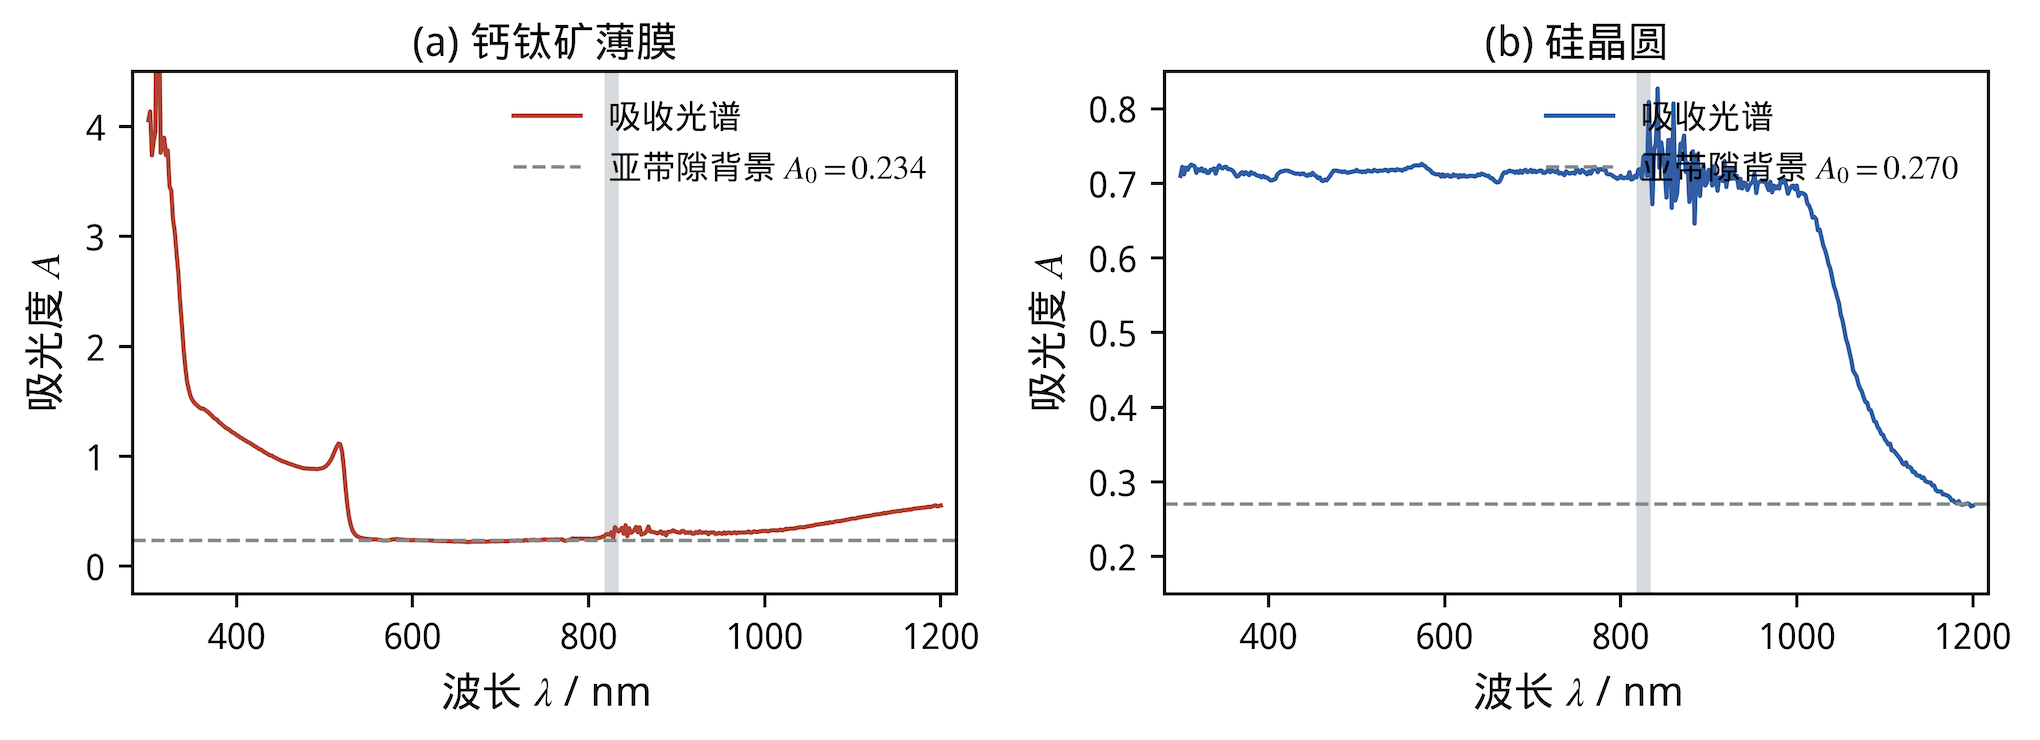
\includegraphics[width=\textwidth]{images/image-2026-11-01-16-36-21.png}
\caption{样品吸收光谱：（a）钙钛矿薄膜；（b）硅晶圆。虚线为亚带隙背景 $A_0$，灰色区为探测器/光栅切换波段。}
\label{fig:abs}
\end{figure}

\subsection*{3. Tauc plot 与禁带宽度}

图 \ref{fig:tauc}(a)：钙钛矿薄膜 $(A'h\nu)^2$ 随 $h\nu$ 在吸收边附近近似线性上升，选取
516--528\,nm（$2.349\sim2.403$\,eV，7 个数据点）作线性拟合，得
$(A'h\nu)^2=89.4\,(h\nu-2.348)$，$R^2=0.962$，横轴截距
\begin{equation}
E_g(\text{钙钛矿})=2.35\ \mathrm{eV}.
\end{equation}

图 \ref{fig:tauc}(b)：硅晶圆 $(A'h\nu)^{1/2}$ 在吸收边区线性良好，选取
1026--1104\,nm（$1.123\sim1.209$\,eV，40 个数据点）作线性拟合，得
$(A'h\nu)^{1/2}=4.49\,(h\nu-1.060)$，$R^2=0.9950$，横轴截距
\begin{equation}
E_g(\text{硅})=1.06\ \mathrm{eV}.
\end{equation}

\begin{table}[htbp]
\centering
\caption{Tauc 外推结果汇总}
\label{tab:eg}
\begin{tabular}{@{}lccccccc@{}}
\toprule
样品 & 跃迁类型 & $n$ & $A_0$ & 拟合区间 & 点数 & $R^2$ & $E_g$\,/eV \\
\midrule
钙钛矿薄膜 & 直接带隙 & 1/2 & 0.234 & 2.349--2.403\,eV (516--528\,nm) & 7  & 0.962  & 2.35 \\
硅晶圆     & 间接带隙 & 2   & 0.270 & 1.123--1.209\,eV (1026--1104\,nm) & 40 & 0.9950 & 1.06 \\
\bottomrule
\end{tabular}
\end{table}

\begin{figure}[htbp]
\centering
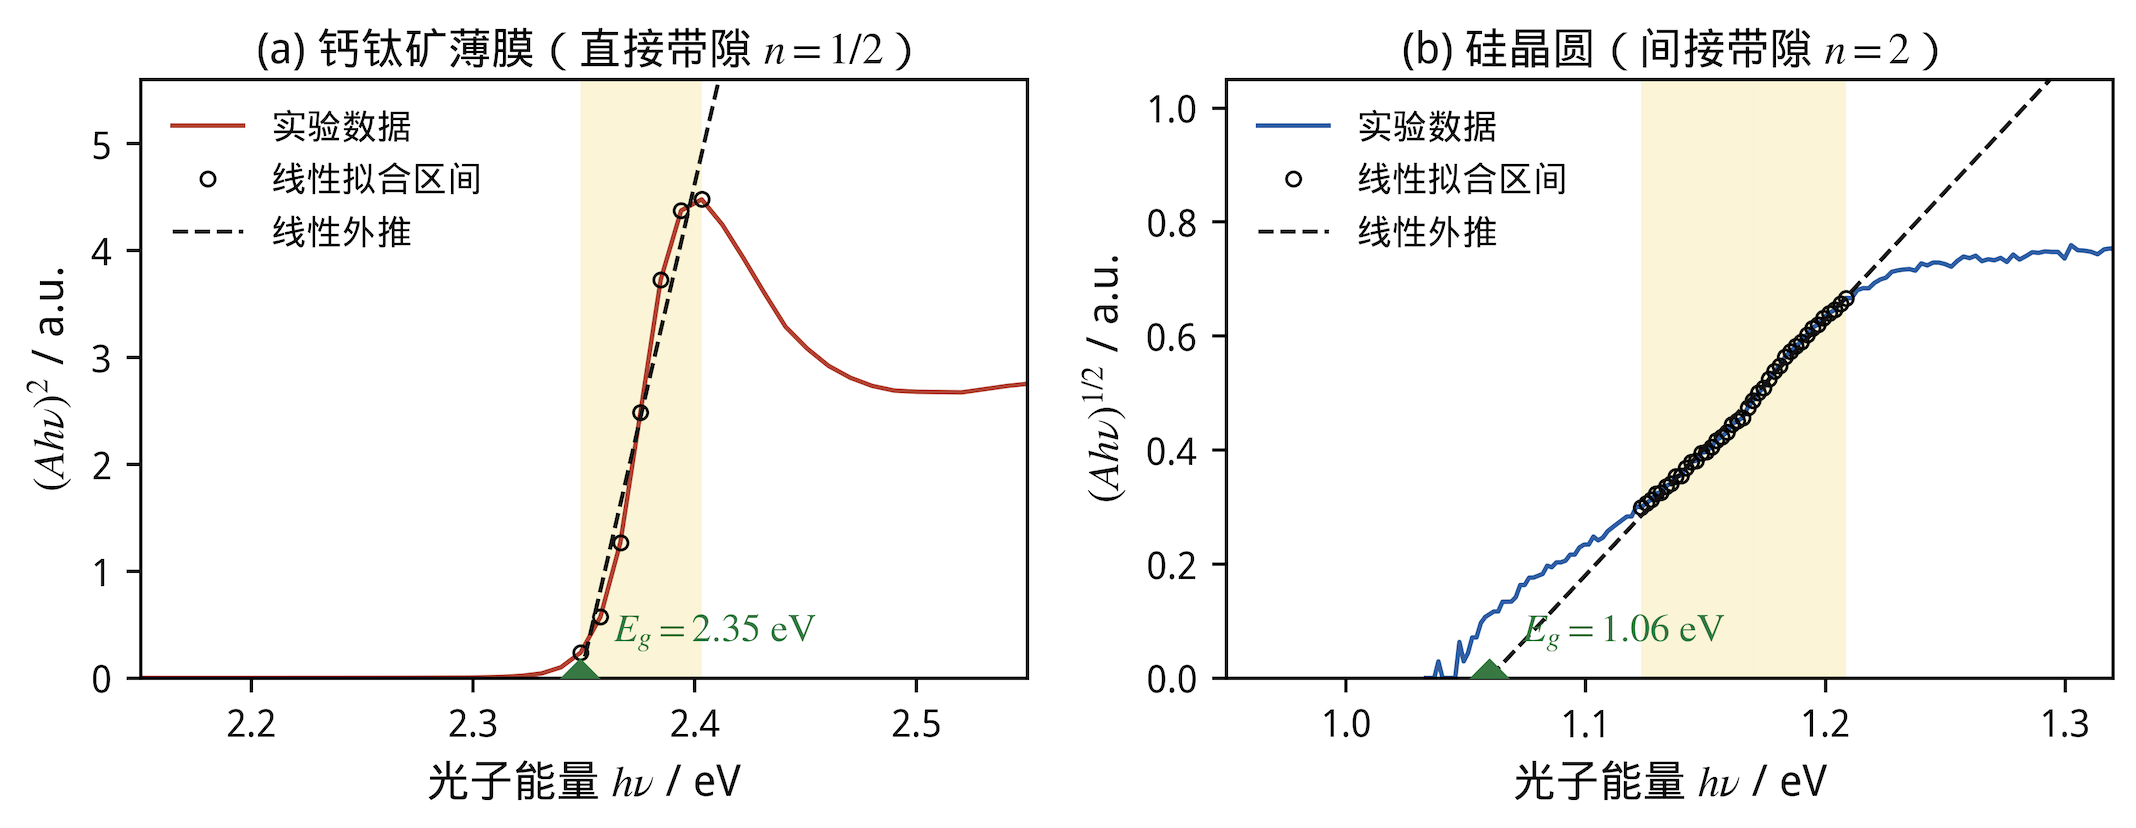
\includegraphics[width=\textwidth]{images/image-2026-11-01-16-35-23.png}
\caption{Tauc plot 与线性外推：（a）钙钛矿薄膜 $(A'h\nu)^2$--$h\nu$；（b）硅晶圆 $(A'h\nu)^{1/2}$--$h\nu$。
黄色区为线性拟合区间，黑色虚线为最小二乘直线及其外推，绿色菱形为横轴截距 $E_g$。}
\label{fig:tauc}
\end{figure}

\begin{figure}[htbp]
\centering
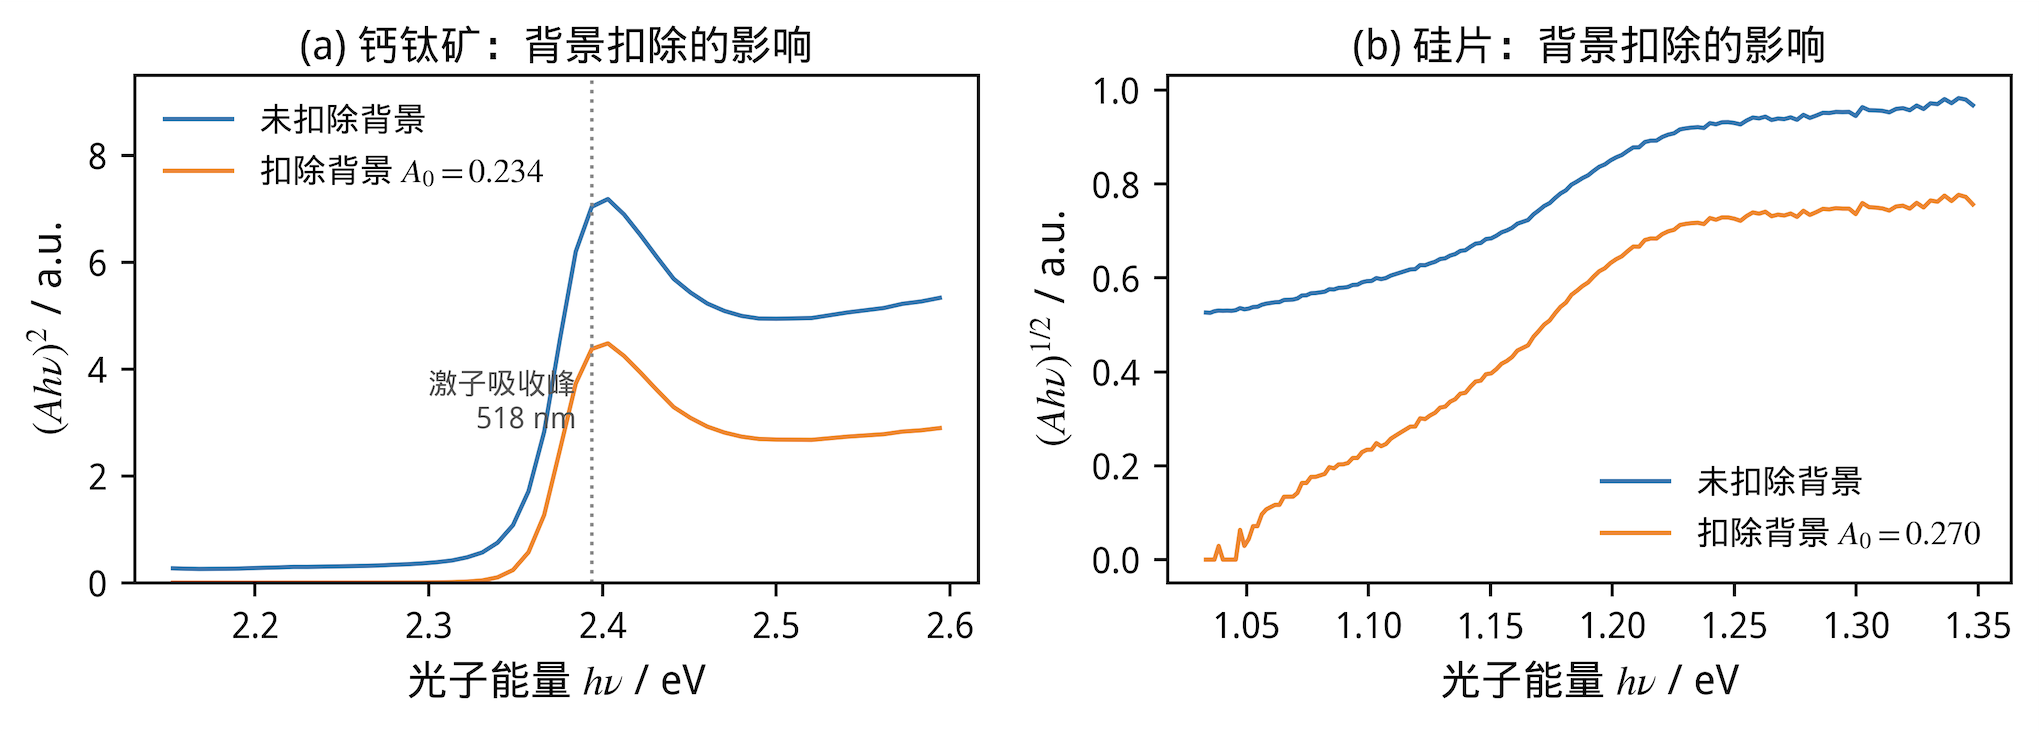
\includegraphics[width=\textwidth]{images/image-2026-11-01-16-35-46.png}
\caption{亚带隙背景扣除对 Tauc 图的影响：（a）钙钛矿薄膜；（b）硅晶圆。}
\label{fig:bg}
\end{figure}

\section*{实验结论（20分）}

采用光吸收系数法（Tauc 外推）测得：钙钛矿薄膜为直接带隙半导体，$E_g=2.35$\,eV；
硅晶圆为间接带隙半导体，$E_g=1.06$\,eV，与文献值 1.12\,eV 相差 5.4\%，在本实验误差范围内。
结果验证了 $(\alpha h\nu)^{1/n}$--$h\nu$ 关系中指数 $n$ 对直接/间接跃迁的区分作用。


\section*{实验启示和拓展（10分）}

\textbf{（1）与文献值比较。}硅在 300\,K 的间接带隙为 1.12\,eV，本实验得 1.06\,eV，相对偏差 $-5.4\%$；
钙钛矿得 2.35\,eV，与宽禁带溴基钙钛矿（MAPbBr$_3$ 约 2.3\,eV、CsPbBr$_3$ 约 2.36\,eV）一致，
其激子吸收峰位（516\,nm）亦与该体系相符。

\textbf{（2）背景扣除的必要性。}图 \ref{fig:bg} 给出扣除与不扣除背景的 Tauc 图对比：硅片不扣背景时截距
降至 0.92\,eV（相对偏低约 13\%），而钙钛矿仅由 2.35\,eV 变为 2.34\,eV。原因是硅的吸收边区吸光度
（0.3--0.7）与背景（0.27）量级相当，背景占比大；钙钛矿拟合区吸光度远大于背景，影响可忽略。
可见对弱吸收边样品必须作背景扣除。

\textbf{（3）拟合窗口的依赖性。}吸收边附近存在 Urbach 尾与激子峰，Tauc 曲线略呈弯曲，截距随窗口选取而变：
钙钛矿窗口由 2.32--2.40\,eV 移至 2.35--2.40\,eV 时 $E_g$ 由 2.34\,eV 变至 2.35\,eV；
硅片窗口由 1.05--1.21\,eV 移至 1.12--1.21\,eV 时 $E_g$ 由 1.04\,eV 变至 1.06\,eV。由此估计窗口引入的
不确定度约 $\pm0.02$\,eV。

\textbf{（4）其他误差来源。}硅片强吸收区吸光度饱和，可用数据集中于吸收边，使外推结果对 $A_0$ 与窗口较敏感；
狭缝宽度 2.0\,nm 与 2\,nm 采样间隔在吸收边处对应能量分辨率约 0.004--0.01\,eV；样品未作反射校正，
膜厚不均与表面散射亦会带来偏差。

\end{document}